\scanpage{38}
\mspage{19}
\[
(67)\qquad u(\widetilde d_i^{\prime\omega})=\varphi_i^{\omega'}(\underbrace{\xi'}_{\eta\xi})\widetilde d_i^{\prime\omega}
\]
On a aussi des chemins
\diagram{\begin{tikzcd}[ampersand replacement=\&,column sep=large,row sep=large]
P^\omega\arrow[rr,"d_i^\omega"]\arrow[dr,"d_{\omega'i}^\omega"']\&\&R_i^\omega\\
\&Q_{\omega'i}\arrow[ur,"c_{\omega'i}^{\omega'}"']\&
\end{tikzcd}}\quad(66')
\[
d_i^\omega=c_{\omega'i}^{\omega'}\cdot d_{\omega'i}^\omega
\]
\margin{\diagram{\begin{tikzcd}[ampersand replacement=\&,column sep=small,row sep=large]
\&P_\infty^\omega\arrow[d,"d_{\omega'i}^\omega"]\arrow[dl,dashed]\\
R_i^\omega\&Q_{\omega'i}\arrow[l,bend left=15,"c_{\omega'i}^{\omega'}"]
\end{tikzcd}}}
\margin{NB $\tau(d_i^\omega)=d_i^{\prime\omega}$}
et on aura également
\[
(67')\qquad u(\widetilde d_i^\omega)=\varphi_i^\omega(\eta\widetilde\sigma_\infty(\xi))\widetilde d_i^\omega
\]
\figure{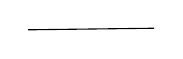
\begin{tikzpicture}\draw (0,0)--(1.6,.02);\end{tikzpicture}}

Je vois encore deux cas à regarder, savoir les sous-groupoïdes pleins de $\mathrm{VI}$ induits sur les \inserted{huit} sommets $(R_{i,\omega},P^\omega)$, soit $\mathrm{VII}$, décrit par le graphe de $=$ nom et les flèches $d_i^{\prime\omega},d_i^\omega,a_i^\omega,b_i^\omega$ (24 flèches), et celui induit sur les \deleted{cinq points} \inserted{sommets} $Q_i,P^\omega$ --- à strictement parler, c'est le groupoïde déjà nommé $\mathrm{IV}$ ayant les $\unsure{\Rightarrow|=}$ \deleted{\unsure{dits}} sommets, mais
\figure{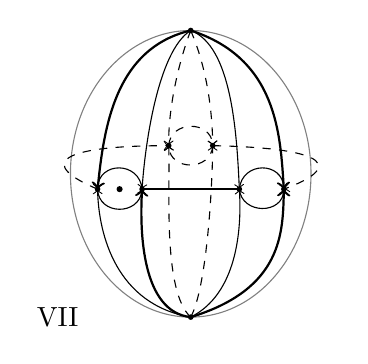
\begin{tikzpicture}[scale=.65]
\draw[gray] (0,0) ellipse (2.35 and 2.8);
\coordinate (P) at (0,2.8);\coordinate (M) at (0,-2.8);
\coordinate (A) at (-1.82,-.3);\coordinate (B) at (-.95,-.3);
\coordinate (C) at (-.43,.55);\coordinate (D) at (.43,.55);
\coordinate (E) at (.95,-.3);\coordinate (F) at (1.82,-.3);
\foreach \p in {P,M,A,B,C,D,E,F}{\fill (\p) circle (.055);}
\draw[thick,->] (P)..controls (-1.5,2.45) and (-1.7,.85)..(A);
\draw[->] (P)..controls (-.65,2.4) and (-.9,.5)..(B);
\draw[dashed,->] (P)..controls (-.25,2.15) and (-.44,1.25)..(C);
\draw[dashed,->] (P)..controls (.3,2.1) and (.42,1.3)..(D);
\draw[->] (P)..controls (.8,2.5) and (.9,.8)..(E);
\draw[thick,->] (P)..controls (1.7,2.25) and (1.75,.75)..(F);
\draw[->] (M)..controls (-1.45,-2.55) and (-1.8,-1.2)..(A);
\draw[thick,->] (M)..controls (-.95,-2.7) and (-1,-1.15)..(B);
\draw[dashed,->] (M)..controls (-.55,-2.3) and (-.4,-.3)..(C);
\draw[dashed,->] (M)..controls (.3,-2.25) and (.42,-.4)..(D);
\draw[->] (M)..controls (.9,-2.35) and (1,-1.1)..(E);
\draw[thick,->] (M)..controls (1.8,-2.25) and (1.8,-1.15)..(F);
\draw[<-] (B)..controls (-1,-.82) and (-1.8,-.82)..(A);
\draw[->] (B)..controls (-1,.25) and (-1.8,.25)..(A);
\draw[dashed,->] (C)..controls (-.4,1.05) and (.4,1.05)..(D);
\draw[dashed,->] (D)..controls (.4,.05) and (-.4,.05)..(C);
\draw[->] (E)..controls (1,.25) and (1.8,.25)..(F);
\draw[->] (E)..controls (1,-.8) and (1.8,-.8)..(F);
\draw[thick] (B)--(E);
\draw[dashed,->] (A)..controls (-3,.2) and (-2.6,.55)..(C);
\draw[dashed,->] (D)..controls (2.85,.5) and (2.9,.1)..(F);
\fill (-1.39,-.3) circle (.06);
\node at (-2.6,-2.8) {$\mathrm{VII}$};
\end{tikzpicture}}
\margin{\uline{NB} les $b_i^\omega$ reliant directement les $\unsure{Q_i|R_i}$ sont ici inutiles}
\figure{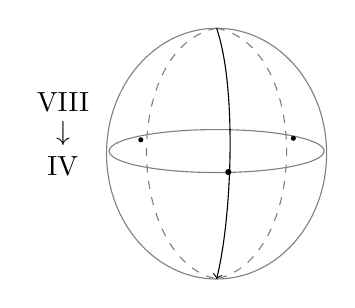
\begin{tikzpicture}[scale=.65]
\draw[gray] (0,0) ellipse (2.15 and 2.45);
\draw[gray] (0,.05) ellipse (2.1 and .42);
\draw[gray,dashed] (0,2.45)..controls (-1.85,2.1) and (-1.8,-2.05)..(0,-2.45);
\draw[gray,dashed] (0,2.45)..controls (1.85,2.1) and (1.8,-2.05)..(0,-2.45);
\draw[->] (0,2.45)..controls (.4,1.3) and (.3,-1.25)..(0,-2.45);
\fill (-1.48,.27) circle (.05);\fill (1.5,.3) circle (.05);\fill (.23,-.36) circle (.06);
\node at (-3,1) {$\mathrm{VIII}$};\node at (-3,.4) {$\unsure{\downarrow}$};\node at (-3,-.25) {$\mathrm{IV}$};
\end{tikzpicture}}
représenté par un graphe un peu plus grand --- dans $\boxed{\mathrm{VIII}}$ on distingue les \inserted{six} \deleted{flèches} $d_i^\omega$ seulement, et on en donne \unsure{par} en plus les $\widetilde a_i^\omega$, ce qui est inutile en fait par (35). (Donc il n'est pas étonnant que dans (37), la donnée de $\widetilde\alpha$, qui
\margin{37}
